% This is samplepaper.tex, a sample chapter demonstrating the
% LLNCS macro package for Springer Computer Science proceedings;
% Version 2.21 of 2022/01/12
%
\documentclass[runningheads,UKenglish]{llncs}
%
\usepackage[T1]{fontenc}
% T1 fonts will be used to generate the final print and online PDFs,
% so please use T1 fonts in your manuscript whenever possible.
% Other font encondings may result in incorrect characters.
%
\usepackage{graphicx}
% Used for displaying a sample figure. If possible, figure files should
% be included in EPS format.
\usepackage{amsmath,amssymb,amsfonts}
\usepackage{algorithmic}
\usepackage{graphicx}
\usepackage[tworuled,algosection,figure,linesnumbered]{algorithm2e}
\usepackage{textcomp}
\usepackage{xcolor}
\usepackage{paralist}
\usepackage{url}
\usepackage{hyperref}
\usepackage{booktabs}
%\usepackage{cprotect}
%\usepackage{caption}
\usepackage{subcaption}
%\captionsetup{belowskip=0pt}
\usepackage{float}
% Cool diagrams
\usepackage{tikz}
\usetikzlibrary{positioning,quotes,shapes.geometric,arrows.meta}
\pgfdeclarelayer{nodelayer} 
\pgfdeclarelayer{edgelayer}
\pgfdeclarelayer{embeded}
\pgfdeclarelayer{stages}
\pgfsetlayers{main,nodelayer,edgelayer,stages,embeded}
\tikzstyle{new style 0}=[fill=white, draw=black, shape=circle, align=center]
\tikzstyle{tree_edge}=[-, draw=black]
\tikzstyle{opChan}=[-Stealth, black]
\tikzstyle{daChan}=[-Stealth, red]
\tikzstyle{io}=[trapezium, trapezium angle=67, trapezium stretches body, fill=blue!30, draw=black, thick]
\tikzstyle {filter_gen} = [rectangle, rounded corners, text centered, draw=black, fill=blue!30, thick]
\tikzset{
  invisible/.style={opacity=0},
  visible on/.style={alt={#1{}{invisible}}},
  alt/.code args={<#1>#2#3}{%
    \alt<#1>{\pgfkeysalso{#2}}{\pgfkeysalso{#3}} % \pgfkeysalso doesn't change the path
  },
}

%
% If you use the hyperref package, please uncomment the following two lines
% to display URLs in blue roman font according to Springer's eBook style:
\usepackage{color}
\renewcommand\UrlFont{\color{blue}\rmfamily}
%

\graphicspath{{./figs/}} %helpful if your graphic files are in another directory

\newcommand{\instancename}{DP-Instance}
\newcounter{instance}

\newcommand{\mst}{$\mathsf{MST}$}
\newcommand{\msts}{$\mathsf{MST}$s}
\newcommand{\mstof}[1]{$\mathsf{MST}_{#1}$}
\newcommand{\dynmst}{\mathsf{Dynamic\_MST}}
\newcommand{\dpm}{$\mathsf{DPM}$}
\newcommand{\DP}{$\mathsf{DP}$}
%\newcommand{\DPmst}{$\mathsf{DP_{KRUSKAL}}$}
%\newcommand{\DPmstv}[1]{$\mathsf{DP_{KRUSKAL\_{#1}}}$}
%\newcommand{\DPmst}{$\mathsf{DP\_{Kruskal}}$}
%\newcommand{\DPmstv}[1]{$\mathsf{DP\_{Kruskal\_{#1}}}$}
\newcommand{\DPmst}{\texttt{DP\_{Kruskal}}}
\newcommand{\DPmstv}[1]{\texttt{DP\_{Kruskal\_{#1}}}}
\newcommand{\FKruskal}{\texttt{Filter\_{Kruskal}}}
\newcommand{\Kruskal}{\texttt{Kruskal}}

\newcommand{\Go}{{\tt Go}}
\newcommand{\Golang}{{\tt Golang}}


\newcommand{\AD}[1]{{\color{red} AD: #1}}
\newcommand{\DB}[1]{{\color{blue} DB: #1}}
\newcommand{\EP}[1]{{\color{magenta} EP: #1}}

\newcommand{\remove}[1]{}

\begin{document}
%
\title{\DPmst: a concurrent algorithm to maintain dynamically minimum spanning trees}
%\thanks{This work has been supported by funds from \ldots}}
%
\titlerunning{\DPmst}
% If the paper title is too long for the running head, you can set
% an abbreviated paper title here
%

\author{Daniel Benedí\orcidID{0009-0005-4295-9484} \and Amalia Duch\orcidID{0000-0003-4371-1286} \and
Edelmira Pasarella\orcidID{0000-0001-8315-4977} \and Cristina Zoltan\orcidID{0000-0001-5303-6371}
}
%
\authorrunning{D. Benedí et al.}
% First names are abbreviated in the running head.
% If there are more than two authors, 'et al.' is used.
%
\institute{Computer Science Department,\\ 
Universitat Polit\`ecnica de Catalunya\\
Barcelona Tech\\
\email{daniel.benedi@estudiantat.upc.edu,\{duch, edelmira\}@cs.upc.edu}}
%
\maketitle              % typeset the header of the contribution
%
\begin{abstract}
We introduce a parallel, distributed and concurrent adaptation of Kruskal algorithm (the \DPmst\ algorithm) that keeps the input graph distributed 
along a pipeline and computes online its minimum spanning tree (or forest).
We provide a working implementation in the \Go\ programming language that, due to its communication channels and co-routines, fits naturally to our algorithm.
We show experimentally that \DPmst\ scales well to a large number of processes 
and that it is competitive against the classic sequential Kruskal algorithm 
and the parallelized version of the \FKruskal\ algorithm.
Our experimental study is done for a large class of dynamic random graphs --including several densities and sizes-- and some real dynamic graphs and 
it reveals that \DPmst\ is also competitive to maintain the minimum spanning tree of dynamic graphs.
\keywords{Spanning trees \and  Parallel algorithms 
\and Concurrency \and Dynamic pipelines \and  Dynamic graphs.}
\end{abstract}
%
\section{Introduction}
\label{sec:intro}

The problem of finding the minimum spanning tree (\mst) of a graph is a well known problem in graph theory with many practical applications. 
In order to improve the efficiency of classical sequential minimum spanning tree algorithms several ways to parallelize them have been studied leading 
to several  algorithms~\cite{bader2006fast,durbhakula2020parallel,tripathy2013new}.
Independently of the topology of the input graphs, all these algorithms 
are generally designed for working either on \textit{in-memory} and/or on static graphs --contrary to dynamic ones. 
Moreover, since usually the size of nowadays graphs don't fit 
into the memory of one processor, algorithms capable 
to work in distributed memory settings are essential in the quest 
to find an efficient solution to the minimum spanning tree problem. 

In this work, we provide a Kruskal-based parallel 
and concurrent algorithm: \DPmst, defined on the 
Dynamic Pipeline Model(\dpm)~\cite{Pasarella2024,DP2019,pasarella2017comparing}. Besides, we show experimentally that \DPmst\ is 
competitive in practice --specially when dealing with dense graphs, 
where other algorithms fail.

Moreover, the \DPmst\ algorithm is suitable to compute the $\dynmst$ of a fully dynamic graph as well as to maintain it actualised by computing efficiently every update on it.
Under this framework the computation of the  $\dynmst$ problem 
turns out to be more natural and intuitive
as well as  more efficient in several cases since the \DPmst\ algorithm discards --early in (and all along) its execution-- several edges.

\vspace{-1em}

\section{The \DPmst\ Algorithm}
\label{sec:DPMST}

\vspace{-0.5em}

A \emph{dynamic pipeline} (DP) consists on different (stateful) stages that run in parallel and are connected  
by means of communication channels that are in charge of the synchronisation of the procedure~\cite{Pasarella2024}. 
The \DPmst\ algorithm distributes the input graph along a DP and there are two types of channels, the event channel and the graph
channel carrying events and \msts, respectively. Figure \ref{fig:dp_example} depicts the state of an instance
of \DPmst. The stages of the DP are defined as follows:

\noindent
\emph{Input ($I$):} Whenever this stage receives an event it passes 
it to the rest of the pipeline through the event channel, if ${\tt op} ={\tt mst}$
it also passes the empty set through the graph channel.\\
%
\noindent
\emph{Output ($O$):} When an event ${\tt mst}$  
arrives to this stage, it outputs the \mstof{G}.\\
%
\emph{Generator ($Gen$):} Whenever an 
event $({\tt op,e=\{v,w\}})$ arrives to this stage  
by the event channel, if ${\tt op}\in\{{\tt insert, update}\}$, a new instance of
Filter stage, $F(v)$, is spawned and added to the pipeline 
between the last filter and $Gen$. The edge $e$ is stored in the local memory of $F(v)$. Besides, whenever 
${\tt op}={\tt mst}$, it passes the \mst\ that arrives by the graph channel 
to the output stage $O$.\\
%
\noindent
\emph{Filter ($F(v)$)}: The parameter $v$ is called the \emph{root} of the 
filter stage. Whenever an event $({\tt op,e=\{v,w\})}$ arrives to $F(v)$, the following things
can happen:  (i) If ${\tt op}=\{{\tt insert, update, delete}\}$ and $e$ is incident to
the root $v$, the event is treated in $F(v)$ according to ${\tt op}$. On the contrary, if it is not incident, the event is passed through the event channel to the next
stage of the pipeline; (ii) If ${\tt op}={\tt mst}$,  a partial \mst\ is computed and
passed to the rest of the pipeline through the graph channel by 
computing the \mst\ of the graph resulting of the union of the 
\mst\ that arrives through  the graph channel with the tree in $F(v)$. 
%The edges of the filter are stored as a list in increasing order by weight. To compute the new partial \mst\ a Kruskal based algorithm is used exploiting the fact that the \mst\ that arrives is also ordered.
%
\vspace{-2em}
\begin{figure}[H]
    \centering
    %Input Graph
    \begin{subfigure}[b]{0.20\textwidth}
    \centering
    \resizebox{\textwidth}{!}{
    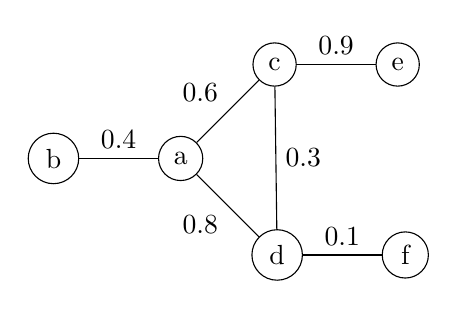
\begin{tikzpicture}
        \begin{pgfonlayer}{nodelayer}
            \node[style=new style 0] (a) at (0,0) {a};
            \node[style=new style 0, left=1cm of a] (b) {b};
            \node[style=new style 0, above right=1.118cm of a] (c) {c};
            \node[style=new style 0, below right=1.118cm of a] (d) {d};
            \node[style=new style 0, right=1cm of c] (e) {e};
            \node[style=new style 0, right=1cm of d] (f) {f};
        \end{pgfonlayer}
        \begin{pgfonlayer}{edgelayer}
            \draw[style={tree_edge}]{} (b) to["0.4"] (a);
            \draw[style={tree_edge}]{} (c) to["0.3"] (d);
            \draw[style={tree_edge}]{} (a) to["0.6"] (c);
            \draw[style={tree_edge}]{} (d) to["0.1"] (f);
            \draw[style={tree_edge}]{} (d) to["0.8"] (a);
            \draw[style={tree_edge}]{} (c) to["0.9"] (e);
        \end{pgfonlayer}
    \end{tikzpicture}
    }    
    \end{subfigure}
    % DP
    \begin{subfigure}[b]{0.5\textwidth}
    \centering
    \resizebox{\textwidth}{!}{
    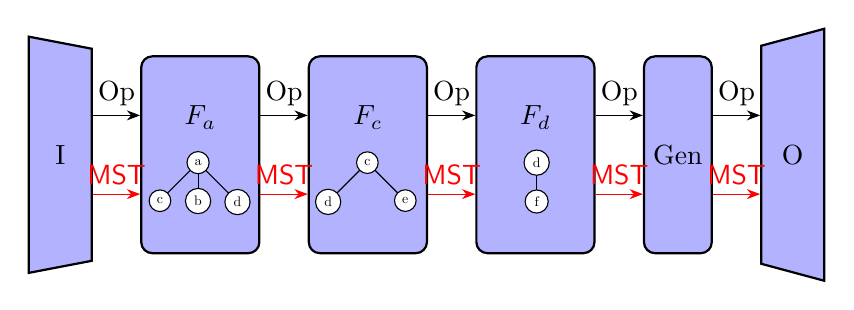
\begin{tikzpicture}
        \begin{pgfonlayer}{nodelayer}
            \node [style=io, minimum height=0.8cm, minimum width=3cm, shape border rotate=270] (In) at (0, 0) {I};
            \node [style=filter_gen, minimum width=1.5cm, minimum height=2.5cm, right= 0.6cm of In,  text depth = 1cm] (F1) {$F_a$};
            \node [style=filter_gen, minimum width=1.5cm, minimum height=2.5cm, right= 0.6cm of F1,  text depth = 1cm] (F2) {$F_c$};
            \node [style=filter_gen, minimum width=1.5cm, minimum height=2.5cm, right= 0.6cm of F2,  text depth = 1cm] (F3) {$F_d$};
            \node [style=filter_gen, minimum width=0.8cm, minimum height=2.5cm, align=center, right= 0.6cm of F3] (Gen) {Gen};
            \node [style=io, minimum height=0.8cm, minimum width=3.2cm, shape border rotate=90, right= 0.6cm of Gen] (Out) {O};
        \end{pgfonlayer}
        \begin{pgfonlayer}{edgelayer}
                \draw [style={opChan}] ([yshift=0.5 cm]Gen.east) to["Op"] ([yshift=0.5 cm]Out.west);
                \draw [style={daChan}] ([yshift=-0.5 cm]Gen.east) to["\mst\ "] ([yshift=-0.5 cm]Out.west);

                \draw [style={opChan}] ([yshift=0.5 cm]In.east) to["Op"] ([yshift=0.5 cm]F1.west);
                \draw [style={daChan}] ([yshift=-0.5 cm]In.east) to["\mst\ "] ([yshift=-0.5 cm]F1.west);
                
                \draw [style={opChan}] ([yshift=0.5 cm]F1.east) to["Op"] ([yshift=0.5 cm]F2.west);
                \draw [style={daChan}] ([yshift=-0.5 cm]F1.east) to["\mst\ "] ([yshift=-0.5 cm]F2.west);
                
                \draw [style={opChan}] ([yshift=0.5 cm]F2.east) to["Op"] ([yshift=0.5 cm]F3.west);
                \draw [style={daChan}] ([yshift=-0.5 cm]F2.east) to["\mst\ "] ([yshift=-0.5 cm]F3.west);
                \draw [style={opChan}] ([yshift=0.5 cm]F3.east) to["Op"] ([yshift=0.5 cm]Gen.west);
                \draw [style={daChan}] ([yshift=-0.5 cm]F3.east) to["\mst\ "] ([yshift=-0.5 cm]Gen.west);
        \end{pgfonlayer}

        \begin{pgfonlayer}{embeded}
            %Filter 1
            \node [style=new style 0, scale=0.5] (a1) at (1.75, -0.1) {a};
            \node [style=new style 0, scale=0.5,below=0.18cm of a1] (b1) {b};
            \node [style=new style 0, scale=0.5,below left=0.4cm of a1] (c1) {c};
            \node [style=new style 0, scale=0.5,below right=0.4cm of a1] (d1) {d};
            \draw[style={tree_edge}]{} (a1) to (b1);
            \draw[style={tree_edge}]{} (a1) to (c1);
            \draw[style={tree_edge}]{} (a1) to (d1);
            
            %Filter 2
            \node [style=new style 0, scale=0.5] (c2) at (3.9, -0.1) {c};
            \node [style=new style 0, scale=0.5,below left=0.4cm of c2] (d2) {d};
            \node [style=new style 0, scale=0.5,below right=0.4cm of c2] (e2) {e};
            \draw[style={tree_edge}]{} (c2) to (d2);
            \draw[style={tree_edge}]{} (c2) to (e2);
            
            %Filter 3
            \node [style=new style 0, scale=0.5] (d3) at (6.05, -0.1) {d};
            \node [style=new style 0, scale=0.5,below=0.18cm of d3] (f3) {f};
            \draw[style={tree_edge}]{} (d3) to (f3);
        \end{pgfonlayer}
    \end{tikzpicture}
    }
    \end{subfigure}
    %\hfill
    %Output MST
    \begin{subfigure}[b]{0.20\textwidth}
    \centering
    \resizebox{\textwidth}{!}{
    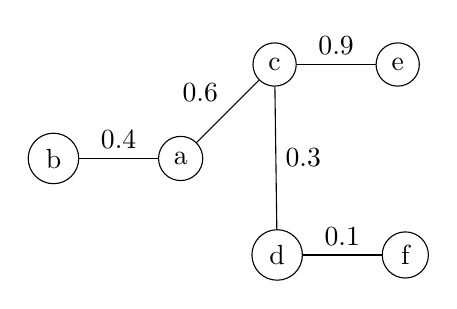
\begin{tikzpicture}
        \begin{pgfonlayer}{nodelayer}
            \node[style=new style 0] (a) at (0,0) {a};
            \node[style=new style 0, left=1cm of a] (b) {b};
            \node[style=new style 0, above right=1.118cm of a] (c) {c};
            \node[style=new style 0, below right=1.118cm of a] (d) {d};
            \node[style=new style 0, right=1cm of c] (e) {e};
            \node[style=new style 0, right=1cm of d] (f) {f};
        \end{pgfonlayer}
        \begin{pgfonlayer}{edgelayer}
            \draw[style={tree_edge}]{} (b) to["0.4"] (a);
            \draw[style={tree_edge}]{} (c) to["0.3"] (d);
            \draw[style={tree_edge}]{} (a) to["0.6"] (c);
            \draw[style={tree_edge}]{} (d) to["0.1"] (f);
            \draw[style={tree_edge}]{} (c) to["0.9"] (e);
        \end{pgfonlayer}
    \end{tikzpicture}
    }    
    \end{subfigure}
    \caption{\label{fig:dp_example} A \DPmst\ at some point of its execution, the input graph and the \mst\ that it returns. The graph is distributed along filters $F_a$, $F_c$ and $F_d$.} 
\end{figure}
%
\vspace{-3em}
\section{Implementation and Experiments}
\label{sec:experiments}
%
As is standard in parallel applications~\cite{bader2002algorithm}, we recorded the elapsed
wall-clock time $T(k,n,m)$—the time elapsed from the start of the execution of \DPmst\ by the first processor until its end by the last
processor—for a graph with $n$ vertices and $m$ edges using
$k$ processors. Notably, all experiments assumed no prior knowledge of the incoming graph, unlike the classic
fully dynamic model where the number of vertices is known in advance, allowing ad-hoc optimizations. 

%\subsection{Static \mst\ on random graphs}
%

\noindent
\textbf{Static \mst\ on random graphs.} 
We generated random graphs where each edge has a probability $p$ of being present, as introduced
by Gilbert~\cite{gilbert1959}. Instead of visiting every edge individually, we used Batagelj's 
method~\cite{Batagelj2005}, which involves generating a random number to determine how many edges
to skip based on the probability $p$. For each combination of nodes ($10^3, 2\cdot10^3, 10^4, 5\cdot10^4$)
and edge probability ($0.10, 0.25, 0.50, 0.75, 0.9$), 20 random graphs were generated.
%
\iffalse
\begin{figure}[H]
\begin{center}
    \includegraphics[width=0.9\textwidth]{figs/SomeDensities_mixed.pdf}
\end{center}
\caption{\label{fig:dpmst-versions}Comparison of \DPmst\ with different root numbers per filter: \DPmstv{const(10)}, \DPmstv{log}, and \DPmstv{sqrt}; and with other algorithms on a single core.}
\end{figure}
\fi

%\vspace{-1em}
\begin{figure}%[H]
\begin{center}
    \begin{subfigure}{\textwidth}
    \centering
    \includegraphics[width=\textwidth]{figs/SomeDensities_mixed.pdf}
    \caption{\label{fig:dpmst-versions}Comparison of \DPmst\ with \DPmstv{const(10)}, \DPmstv{log}, \DPmstv{sqrt}, {\tt Prim} and \FKruskal\ on a single core.}
    \end{subfigure}
    
    \begin{subfigure}{\textwidth}
    \centering
    \includegraphics[width=\textwidth]{figs/SpeedUpDPandFK_sample.pdf}
    \caption{\label{fig:speedup_dp_fk}A comparison of the speed-ups of \DPmst\ and \FKruskal\ in multicore.}
    \end{subfigure}
    \caption{Experimental results on static random graphs.}
\end{center}

\end{figure}
%
\vspace{-2em}
\noindent
To study the effect of the number of roots in each filter, we consider three
options: a constant number of roots \DPmstv{const},  $\log(n)$ roots \DPmstv{log}, and $\sqrt{n}$ roots
\DPmstv{sqrt} on a single core (where $n$ is the number of vertices of the input graph).  We also compared \DPmst\ with \FKruskal~\cite{Osipov2009},
and a message-passing {\tt Prim}~\cite{Loncar2014} implementation. \FKruskal\ was chosen for its simple
parallelization, while the {\tt Prim} algorithm was selected for using the same type of parallelism as \DPmst, 
with results taken from their paper. Experimental results in Figure~\ref{fig:dpmst-versions} show that 
for small graphs, \FKruskal\ is 
faster while as graph size and density increase, \DPmstv{sqrt}\ becomes the best option. %{\tt Prim} 
%algorithm has too much communication overhead to be competitive.
\iffalse
\begin{figure}[H]
\begin{center}
    \includegraphics[width=0.8\textwidth]{figs/SomeDensities_mixed.pdf}
\end{center}
\caption{\label{fig:dpmst-versions}Comparison of \DPmst\ with different root numbers per filter: \DPmstv{const(10)}, \DPmstv{log}, and \DPmstv{sqrt}; and with other algorithms on a single core.}
\end{figure}
\fi
%
\iffalse
\begin{figure}[H]
\begin{center}
    \includegraphics[width=\textwidth]{figs/SpeedUpDPandFK_sample.pdf}
\end{center}
\caption{\label{fig:speedup_dp_fk}A comparison of the speed-ups of the \DPmst\ and the  \FKruskal\ algorithms in a multi core setup.}
\end{figure}
\fi
%
%\vspace{-1em}
\noindent
Figure~\ref{fig:speedup_dp_fk} compares different versions of \DPmst\ with parallelized \FKruskal\
on a multi-core set-up. We calculated absolute speedup as the execution time of the sequential 
implementation divided by the parallel implementation $T(k,n,m)$. For graphs with a small expected number
of edges, parallel \FKruskal\ can outperform any \DPmst\ variant. 
As graph density or the 
number of vertices increases to real-world sizes, \DPmst\ significantly outperforms \FKruskal\ in 
both speedup and efficiency. 
%Due to hardware limitations, we couldn't experimentally reach the number 
%of processors needed to observe the algorithms' speed stagnation.
%
\iffalse
\begin{figure}[H]
\begin{center}
    \includegraphics[width=\textwidth]{figs/SpeedUpDPandFK_sample.pdf}
\end{center}
\caption{\label{fig:speedup_dp_fk}A comparison of the speed-ups of the \DPmst\ and the  \FKruskal\ algorithms in a multi core setup.}
\end{figure}
\fi

%
%\subsection{Dynamic \mst\ on real graphs}
%\vspace{-1em}
\noindent
\textbf{Dynamic \mst\ on real graphs}. We compare \DPmst\ and \FKruskal\ on realistic dynamic graphs obtained from \href{https://DynGraphLab.github.io/}{\texttt{https://DynGraphLab.github.io/}}~\cite{HanHenSchuSurvey2021}.
After each operation of insertion or deletion of an edge, we have asked in for an actualisation of the \mst. In Table \ref{tab:real_graphs_time}, we observe that \DPmst\ is effective for maintaining the \mst. Figure \ref{fig:real_graphs_speed} demonstrates its excellent performance in a parallel environment, showcasing significant scalability.

\vspace{-1.65em}

\begin{figure}
    \centering
    \begin{subfigure}{\textwidth}
     \centering
        \resizebox{0.65\textwidth}{!}{%
        \begin{tabular}{lcccc}
            \toprule
            Dataset & $n$ & op. & \FKruskal & \DPmst\ \\
            \midrule
            {\tt as-caida}     &31379 &119468&  1h 30min &  1h 19min \\
            {\tt movielens10m} &49847&384585&  1h 39min &  1h 20min \\
            {\tt simplewiki}   &100312&889016 &17h  8min & 11h 29min \\
            \bottomrule
        \end{tabular}
        }
        \caption{\label{tab:real_graphs_time}Time, 1 core, 10 roots per filter}
    \end{subfigure}
%\end{figure}
   % \hfill

 %\begin{figure}[t]
  \centering
    \begin{subfigure}{\textwidth}
    \centering
        \includegraphics[width=0.84\textwidth]{figs/RealGraphs.pdf}
        \caption{\label{fig:real_graphs_speed}Multicore comparison of speed-ups}        
   \end{subfigure}
    \caption{\label{fig:real-graphs}Experimental results on real dynamic graphs where $n$ is the number of vertices and op. the number of operations.}
\end{figure}
%
\vspace{-2em}

\noindent
Experiments were run at the RDLab-UPC cluster~\href{https://rdlab.cs.upc.edu/}{\texttt{https://rdlab.cs.upc.edu/}}
across different nodes with various cores: Intel Xeon: E5-2450 (16),
X5675 (12), X5670 (12), X5660 (12),
and X5550 (8). Jobs ran with 16GB of RAM and a variable
number of cores depending and executed 10 times, average
time was reported, with a 24-hour timeout \DPmst\ uses \Golang\ 1.20. Available on \href{https://github.com/danielbenedi6/MasterThesis}{https://github.com/danielbenedi6/MasterThesis}.
%
\vspace{-1em}

\section{Final Remarks}
\label{sec:ongoing}
%We propose the \DPmst\ algorithm and we implemented it in \Go\ for its efficient handling of dynamic pipelines. 
We propose the \DPmst\ algorithm. Our preliminary experiments on various random and real graphs demonstrate that our algorithm is particularly competitive for dense graphs, showing improved performance over the \FKruskal\ algorithm for graphs with over $2 \cdot 10^3$ vertices. It also scales well, enhancing efficiency and speed up to 16 cores. 
%
Future work will involve comparing our algorithm with a {\tt MapReduce}-based competitor~\cite{nowicki2021dynamic} despite not being able to find a working version; evaluating other \mst\ algorithms within the \DPmst\ model; assessing different implementation languages; conducting extensive experiments with larger datasets and testing adaptability to various dynamic graph models.

%
% ---- Bibliography ----
%
% BibTeX users should specify bibliography style 'splncs04'.
% References will then be sorted and formatted in the correct style.
%
\bibliographystyle{splncs04}
\bibliography{biblio}
%
\end{document}